\documentclass[11pt]{article}
\usepackage[a4paper,margin=19mm]{geometry}
\usepackage{fontspec}
\setmainfont{lmroman10-regular.otf}
\usepackage{amsmath,amssymb,amsthm,mathtools,amscd,xcolor,graphicx,hyperref}
\hypersetup{hidelinks}
\numberwithin{equation}{section}
\newtheorem{theorem}{Theorem}[section]
\newtheorem{lemma}[theorem]{Lemma}
\newtheorem{proposition}[theorem]{Proposition}
\newtheorem{corollary}[theorem]{Corollary}
\newtheorem{claim}[theorem]{Claim}
\newtheorem{fact}[theorem]{Fact}
\newtheorem{conjecture}[theorem]{Conjecture}
\theoremstyle{definition}
\newtheorem{definition}[theorem]{Definition}
\newtheorem{example}[theorem]{Example}
\newtheorem{remark}[theorem]{Remark}
\newtheorem{question}[theorem]{Question}
\theoremstyle{plain}
\newcommand{\C}{\mathbb C}
\newcommand{\R}{\mathbb R}
\newcommand{\Q}{\mathbb Q}
\newcommand{\Z}{\mathbb Z}
\newcommand{\N}{\mathbb N}
\newcommand{\eee}{\mathrm e}
\newcommand{\cclass}[1]{\textsf{#1}}
\newcommand{\cproblem}[1]{\textsc{#1}}
\newcommand{\ie}{i.\,e.}
\newcommand{\Ie}{I.\,e.}
\newcommand{\eg}{e.\,g.}
\newcommand{\Eg}{E.\,g.}
\newcommand{\phd}{Ph.\,D.}
\newcommand{\msc}{M.\,S.}
\newcommand{\bsc}{B.\,S.}
\newcommand{\expref}[2]{\hyperref[#2]{#1~\ref{#2}}}
\newcommand{\expeqref}[2]{\hyperref[#2]{#1~\eqref{#2}}}
\newcommand{\exprefsilent}[2]{\hyperref[#2]{#1}}
\providecommand{\etal}{et~al.}
\usepackage{eprint}
\usepackage{subcaption,tikz,algorithm2e,aumacros}
\title{Polynomial-time grid-digraph reachability in quarter-power space using pseudoseparators}
\author{Rahul Jain, Raghunath Tewari}
\date{doi:10.4086/toc.2023.v019a002; CC BY 3.0}
\begin{document}
\maketitle
\noindent\textit{Editorial note.} Complete author statement, proof, algorithms, original figures and bibliography retained. Standalone wrapper imports original mathematical packages; unused frontmatter-only orcidlink import omitted.\par\medskip
\noindent\textit{Editorial note.} Original fig\_sep.tex input expanded inline for the existing standalone interface; raw source and original figure TeX retained. Source locators point to the explicitly named render copy.\par\medskip
\noindent\textit{Allowed standard prerequisites (editorial).}\begin{itemize}
\item Directed reachability, planar/grid graphs and asymptotic algorithm analysis. All source-local auxiliary graph, pseudoseparator and implicit recursion definitions retained.. No collector algorithm or repaired argument.
\end{itemize}\medskip
\section{Introduction}
%
%
%
%
%
%
%
%
%
%
%
Let $s$ and $t$ be vertices of a given 
%
directed graph (digraph). %
%
The problem of 
 %
digraph %
reachability is to decide if there is a path from $s$ to $t$. This problem has %
%
many  %
applications in the field of algorithms and computational complexity theory. Many algorithms for network-related problems use it as a subroutine. 
%
Digraph reachability is \textsf{NL}-complete and thus
%
captures  %
the complexity of %
nondeterministic  %
logarithmic space. Hence designing better algorithms for this problem is of utmost importance
%
to the theory of computing.  %

Standard 
 %
traversal algorithms such as DFS and BFS give a
%
linear-time   %
algorithm for this problem, but they require linear space. Savitch's 
divide-and-conquer 
%
algorithm %
solves  %
reachability in $O(\log^2 n)$ space. However, as a tradeoff, it requires $n^{O(\log n)}$ time \cite{Savitch}. Hence it is natural to ask whether we can get the best of both worlds and design an algorithm for 
 %
digraph %
reachability that runs in polynomial time and uses \emph{polylogarithmic} space. Wigderson asked a relaxed version of this question in his survey, whether 
 %
digraph %
reachability can be solved by a polynomial-time algorithm that uses $O(n^{1-\epsilon})$ space \cite{Wigderson}.

Barnes et al.  %
showed that 
%
digraph reachability %
can be decided simultaneously in $n/2^{\Theta(\sqrt{\log n})}$ space and polynomial time \cite{BBRS}. Although this algorithm gives a sublinear %
space bound,  %
it still does not %
answer Wigderson's question.

Undirected graphs can be considered as a specific type of digraphs,
where %
adjacency
%
%
%
%
is a symmetric relation.
Reachability in undirected %
graphs  %
can be solved in logspace \cite{Reingold}. %
%
%
Also, for certain classes of digraphs, where the underlying undirected graph is topologically restricted, we know of polynomial time algorithms with space complexity better than linear. %
%
%
%
Imai et al. presented  
a polynomial-time algorithm that %
solves  %
reachability for planar 
 %
digraphs %
using $O(n^{1/2 + \epsilon})$ space for any $\epsilon >0$ \cite{Imai}. Later, Asano et al. presented a polynomial-time algorithm whose space complexity was $\tilde{O}(n^{1/2})$ for the same problem \cite{Asano}. For 
 %
digraphs %
of higher genus, Chakraborty et al. presented a polynomial-time algorithm that uses $\tilde{O}(n^{2/3}g^{1/3})$ space. Their algorithm additionally requires an embedding of the 
underlying undirected %
graph on a surface of genus $g$, as part of the input \cite{ChakrabortyPavan}. They also gave an $\tilde{O}(n^{2/3})$-space %
algorithm for %
$H$-minor-free   %
 %
digraphs %
which requires
a  %
tree decomposition of the 
underlying undirected %
graph as 
%
part of the %
 input and $O(n^{1/2 + \epsilon})$-space
%
%
%
%
%
%
%
%
%
%
algorithms for
%
%
$K_{3,3}$-minor-free digraphs and for $K_5$-minor-free digraphs. %

For layered planar 
 %
digraphs %
Chakraborty and Tewari showed that for every $\epsilon >0$, there is an $O(n^{\epsilon})$-space %
algorithm \cite{Chakraborty}. Stolee and Vinodchandran presented a polynomial-time algorithm that, for any $\epsilon > 0$ solves \emph{reachability} in 
%
an acyclic digraph %
with $O(n^{\epsilon})$ sources and embedded on the surface of genus $O(n^\epsilon)$ using $O(n^{\epsilon})$ space \cite{Stolee}. For unique-path 
 %
digraphs %
Kannan et al. presented an %
$O(n^{\epsilon})$-space, %
%
polynomial-time algorithm \cite{kannan}.

In this paper, grid 
 %
digraphs %
are our concern. Grid
 %
digraphs %
are a subclass of planar
 %
digraphs. %
In a grid 
 %
digraph, %
%
the  %
vertices are
the %
%
points %
of an $m \times m$ grid.  %
%
The edges can only occur between a vertex and its immediate vertical
%
and  %
horizontal neighbours.  %
We know that reachability in planar 
 %
digraphs %
%
can  %
be reduced to reachability in grid
 %
digraphs %
 in logarithmic space \cite{Allender}. The reduction, however, causes at least a quadratic blow-up in the size of the 
 %
digraph. %
In this paper, we study the simultaneous time--space complexity of reachability in grid graphs.

%
Asano and Doerr presented a polynomial-time algorithm that uses $O(n^{1/2 + \epsilon})$ space for solving reachability in grid 
 %
%
%
%
digraphs  \cite{Asano11}.  %
Ashida and Nakagawa presented an algorithm with improved space complexity of $\widetilde{O}(n^{1/3})$ \cite{AshidaNakagawa}.
%
%
The latter algorithm %
proceeds  %
by first dividing the input grid 
 %
digraph %
into subgrids. It then
%
uses  %
a gadget to transform each subgrid into a planar 
 %
digraph, %
making the whole of the resultant 
 %
digraph %
planar. Finally, it
%
uses  %
the planar reachability algorithm of Imai et al. $\cite{Imai}$ as a subroutine to get the desired space bound.
%

In this paper, we present a $O(n^{1/4 + \epsilon})$ space and polynomial-time algorithm for grid 
 %
digraph %
reachability, thereby significantly improving the
%
space bound  %
of Ashida and Nakagawa.

\begin{theorem}[Main Theorem]
\label{thm:main}
For every $\epsilon > 0$, there exists a polynomial-time algorithm that
%
solves  %
reachability in an %
$n$-vertex   %
grid 
 %
digraph %
using $O(n^{1/4 + \epsilon})$ space.
\end{theorem}


The approach of Ashida and Nakagawa \cite{AshidaNakagawa}
%
%
is   %
to reduce the size of the input $n$-vertex 
 %
digraph %
to a 
 %
digraph %
of size $O(n^{2/3})$. Their new graph %
preserves  %
reachability between vertices and %
is planar.  %
%
They use  %
the planar-reachability algorithm of Asano et al. \cite{Asano}.
%
Our approach is slightly different. We convert the input 
 %
digraph %
into an 
%
\emph{auxiliary digraph} %
 of size $O(n^{1/2 + \alpha/2})$ for arbitrarily small $\alpha$. The auxiliary 
 %
digraph %
is created by dividing the given grid 
 %
digraph %
into subgrids and replacing paths in each subgrid with a single edge between the boundary vertices.  While our auxiliary 
 %
digraph %
preserves reachability, it is not planar; and hence we cannot use Asano et al.'s algorithm directly. The auxiliary 
 %
digraph %
comes with a drawing with
the  %
\emph{crossing property}, that is, if two edges, $e$ and $f$,
%
cross each other in this drawing, there necessarily exist two more edges, one from the tail of $e$ to the head of $f$ and the other from the tail of $f$ to the head of $e$, in the 
 %
digraph. %
This property allows us to use a device that we call \emph{pseudoseparator} to solve reachability in it. A pseudoseparator designates a set of vertices, a set of edges and a set of components of the 
 %
digraph, %
such that a path from one component to %
another   %
necessarily either takes a vertex of the pseudoseparator or crosses one of the edges of the pseudoseparator in the drawing.
We finally solve the problem by recursively solving each of these components and using a traversal algorithm. Due to the crossing property, we are required to store only a small number of vertices for performing the traversal, thereby saving space.

In \expref{Section}{sec:prelims}, we state the definitions and
%
notation  %
that we use in this paper. In \expref{Section}{sec:aux}, we define the auxiliary 
 %
digraph %
and state various properties of it that we use later. In \expref{Section}{sec:pseudosep}, we discuss the concept of the \emph{pseudoseparator}. We give its formal definition and show how to compute the \emph{pseudoseparator} efficiently. In \expref{Section}{sec:auxreach}, we give the algorithm to solve reachability in an auxiliary 
 %
digraph %
and prove its correctness. Finally in \expref{Section}{sec:final} we use the algorithm of \expref{Section}{sec:auxreach} to give an algorithm to decide reachability in grid 
  %
digraphs %
and thus prove \expref{Theorem}{thm:main}.

\section{Preliminaries}
\label{sec:prelims}
Let $[n]$ denote the set $\{0,1,2,\ldots , n\}$. %
%
We denote the vertex set of a 
 %
digraph %
$G$ by $V(G)$ and its edge set by $E(G)$. We assume that the vertices of a 
 %
digraph %
are \emph{indexed} by integers from $1$ to $\lvert V(G) \rvert$. For a subset $U$ of $V(G)$, we denote the %
sub-digraph %
 of $G$ induced by the vertices of $U$ as $G[U]$ and we denote the %
sub-digraph %
 of $G$ induced by the vertices $V(G)\setminus U$ as $G\setminus U$. For a 
 %
digraph %
$G$, %
%
we write $\concom{G}$ to denote  %
the set of all connected components
in the underlying undirected graph of $G$.  %
By
the  %
\emph{underlying undirected graph}, we mean the graph formed by %
symmetrizing the adjacency %
relation.  %
To do this, we consider each directed edge in the digraph and create an undirected edge between the corresponding vertices.
%
%
%
%
Henceforth, whenever we talk about connected components, we will mean the connected components of the underlying undirected graph.
%
In a \emph{drawing} of a graph 
in the plane
we map each vertex to
a  %
point %
in  %
the plane and each edge to a simple arc whose endpoints coincide with the
%
images  %
of the end vertices of the edge.
%
%
%
%
%
Moreover, 
%
the image of a vertex does not belong to the interior of an arc corresponding to any edge. %
We say that a graph is \emph{planar} if there exists a drawing of that graph on a plane such that no two
%
arcs corresponding to the edges %
of the graph %
intersect except at the endpoints. %
Such a drawing is called a \emph{planar embedding}.%

A \emph{planar digraph} is a digraph whose underlying undirected graph is planar. Similarly, a \emph{drawing of a digraph} is defined as the drawing of its underlying undirected graph. %

%
We will represent a planar graph by describing the
%
cyclic  %
ordering of a graph's edges around each vertex. %
 %
%
%
%
%
%
We note that %
%
the results in %
\cite{AllenderMahajan} and \cite{Reingold} %
%
combine to %
a \emph{deterministic logarithmic space} algorithm that decides
whether %
a given graph is planar, and if it is, outputs a planar embedding. Hence, when dealing with planar graphs, we will assume without loss of generality that we have a planar embedding whenever required.   %
%
%
%
%
An  %
$m\times m$
%
\emph{grid digraph} %
is a directed graph %
%
whose 
%
set of vertices is %
$[m] \times [m] = \{0,1,\ldots,m\}\times\{0,1,\ldots,m\}$ so that if $((i_1,j_1),(i_2,j_2)) $ is an edge then $|i_1-i_2|+|j_1-j_2|=1$.  
In other words, we start with an undirected $m\times m$ grid graph. Then, we
%
remove some of the edges and assign directions to the remaining edges while keeping all the vertices. This process results in the formation of an $m\times m$ grid digraph, which has a total of $n=(m+1)^2$ vertices. %
 It follows from the definition that grid 
 %
digraphs %
are %
%
planar.  %
%
%

We will work with $m\times m$ grid 
 %
digraphs %
where $m = O(n^{1/2})$. Hence, a
%
space complexity  %
of $O(m^{1/2 + \epsilon})$ will translate into a space complexity of $O(n^{1/4 + \epsilon'})$ as required.


\section{Auxiliary graph}
\label{sec:aux}
Let $G$ be an $m \times m$ grid 
 %
digraph. %
We divide $G$ into $m^{2\alpha}$ subgrids such that each subgrid is a $m^{1-\alpha} \times m^{1-\alpha}$ grid. Formally, for 
$0 < \alpha < 1$ and %
$1 \leq i,j \leq m^{\alpha}$, the $(i,j)$-th \emph{subgrid} of $G$,
denoted %
$G[i,j]$,  %
is the %
sub-digraph %
of $G$ induced by the set of vertices, $V(G[i,j])$, where $V(G[i, j])$
is %
\[\{(i',j') \mid (i-1)\cdot m^{1-\alpha} \leq i' \leq i\cdot m^{1-\alpha} \textrm{ and } (j-1)\cdot m^{1-\alpha} \leq j' \leq j\cdot m^{1-\alpha} \}\,.\]
%

For ease of presentation, we will assume without loss of generality that variables like $m$ and $\alpha$ are such that the values like $m^{\alpha}$ and $m^{1-\alpha}$ are integers. %


%
%
%
%
We define %
the auxiliary 
 %
digraph %
$\aux{G}[i,j]$ as follows. The vertex set of $\aux{G}[i,j]$ is the set of vertices on the \emph{boundary} of $G[i, j]$. 
%
%
That means, $V(\aux{G}[i,j])$ is
%
\begin{align*}
& \{(i',j') \mid (i',j') \in V(G[i,j]) \textrm{ and }\\
& \ \ ((i-1)\cdot m^{1-\alpha} = i' \textrm{ or } i\cdot m^{1-\alpha} = i' \textrm{ or } (j-1)\cdot m^{1-\alpha} = j' \textrm{ or } j\cdot m^{1-\alpha} = j') \}\,.
\end{align*}
For two vertices $u,v$ in $\aux{G}[i,j]$, $(u,v)$ is an edge in $\aux{G}[i,j]$ if there is a path from $u$ to $v$ in the subgrid $G[i,j]$. 
%
We draw $\aux{G}[i, j]$ on an Euclidean plane by mapping vertex $(x,y)$ to the point with %
coordinates  %
$(x, y)$. The points corresponding to vertices of $\aux{G}[i,j]$ thus lie on a square. We %
use a straight line %
segment  %
to represent the edge if $u$ and $v$ do not lie on a single side
%
%
of this square.  %
and an arc 
%
 inside the
%
square %
to represent it otherwise.  
%

%
We define the %
%
$\alpha$-\emph{auxiliary digraph}, %
$\aux{G}$ as follows. The vertex set of $\aux{G}$, $V(\aux{G}) = \{(i,j) \mid i = k\cdot m^{1-\alpha} \textrm{ or } j = l\cdot m^{1-\alpha}, \textrm{ such that } 0 \leq k,l \leq m^{\alpha} \}$. The edges of $\aux{G}$ are the edges of $\aux{G}[i,j]$ taken over all pairs $(i,j)$. Note that $\aux{G}$ might have parallel edges, since an edge on a side of a block might be %
in the adjacent block as well. In such cases we preserve both the edges,
%
%
in their different blocks of $\aux{G}$ in the drawing of $\aux{G}$ on the plane. \expref{Figure}{fig:auxG} contains an example of a grid 
 %
digraph %
partitioned into subgrids and its corresponding auxiliary 
 %
digraph. %
Since each block $\aux{G}[i,j]$ contains $4m^{1-\alpha}$ vertices, the total number of vertices in $\aux{G}$ %
is  %
at most $4m^{1 + \alpha}$.

Our algorithm for reachability first constructs $\aux{G}$ by solving each of the $m^{1-\alpha} \times m^{1-\alpha}$ grids recursively. It then uses a polynomial-time subroutine to decide reachability in $\aux{G}$. Note that we do not store 
the 
 %
digraph %
$\aux{G}$ explicitly since that would require too much space. Rather we solve a subgrid recursively whenever the subroutine queries for an edge in that subgrid of $\aux{G}$.

Our strategy is to develop a polynomial-time %
algorithm which solves reachability in $\aux{G}$ using $\tilde{O}(\tilde{m}^{1/2 + \beta/2})$ space where $\tilde{m}$ is the number of vertices in $\aux{G}$. As discussed earlier, $\tilde{m}$ %
is %
 at most $4m^{1 + \alpha}$. Hence, the main algorithm requires 
$\tilde{O}(m^{1/2 + \beta/2 + \alpha/2 + \alpha\beta/2})$ space. For a fixed constant $\epsilon > 0$, we can pick $\alpha > 0$ and $\beta > 0$ such that the space complexity becomes $O(m^{1/2 + \epsilon})$.

%
%
%
%

\begin{figure}[ht]
\centering
\begin{subfigure}{0.4\textwidth}
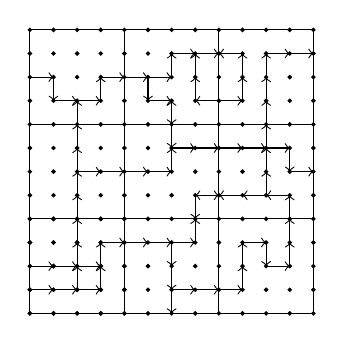
\begin{tikzpicture}[scale = 0.3]

\foreach \x in {0,...,12}
\foreach \y in {0,...,12}
\filldraw (\x,\y) circle (2pt);
\draw[step=4] (0,0) grid (12,12);

\foreach \x in {0,...,4}
\foreach \y in {0,...,4}
\filldraw (\x,\y) circle (2pt);
\draw[step=4] (0,0) grid (4,4);

\draw[->] (0,1) -- (1, 1);
\draw[->] (1,1) -- (2, 1);
\draw[->] (2,1) -- (3, 1);

\draw[->] (0,2) -- (1, 2);
\draw[->] (1,2) -- (2, 2);
\draw[->] (2,2) -- (3, 2);


\draw[->] (3,1) -- (3, 2);
\draw[->] (3,2) -- (3, 3);

\draw[->] (3,3) -- (4, 3);

\draw[->] (2,1) -- (2, 2);
\draw[->] (2,2) -- (2, 3);
\draw[->] (2,3) -- (2, 4);

\draw[->] (4,3) -- (5,3);
\draw[->] (5,3) -- (6,3);
\draw[->] (6,3) -- (7,3);

\draw[->] (6,3) -- (6,2);
\draw[->] (6,2) -- (6,1);
\draw[->] (6,1) -- (6,0);

\draw[->] (7,3) -- (7,4);

\draw[->] (6,1) -- (7,1);
\draw[->] (7,1) -- (8,1);

\draw[->] (8,1) -- (9,1);
\draw[->] (9,1) -- (9,2);

\draw[->] (9,2) -- (9,3);
\draw[->] (9,3) -- (10,3);
\draw[->] (10,3) -- (10,2);
\draw[->] (10,2) -- (11,2);
\draw[->] (11,2) -- (11,3);
\draw[->] (11,3) -- (11,4);

\draw[->] (2,4) -- (2,5);
\draw[->] (2,5) -- (2,6);
\draw[->] (2,6) -- (2,7);
\draw[->] (2,7) -- (2,8);
\draw[->] (2,6) -- (3,6);
\draw[->] (3,6) -- (4,6);

\draw[->] (4,6) -- (5,6);
\draw[->] (5, 6) -- (6,6);
\draw[->] (6,6) -- (6,7);
\draw[->] (6,7) -- (7,7);
\draw[->] (7,7) -- (8,7);
\draw[->] (6,8) -- (6,7);
\draw[->] (8,5) -- (7,5);
\draw[->] (7,5) -- (8,5); %

\draw[->] (7,5) -- (7,4);
\draw[->] (11,4) -- (11,5);
\draw[->] (11,5) -- (10, 5);
\draw[->] (10,5) -- (9,5);
\draw[->] (9,5) -- (8,5);
\draw[->] (10,5) -- (10,6);
\draw[->] (10,6) -- (10,7);
\draw[->] (10,7) -- (10,8);


\draw[->] (8,7) -- (9,7);
\draw[->] (9,7) -- (10, 7);
\draw[->] (10, 7) -- (11,7);
\draw[->] (11, 7) -- (11,6);
\draw[->] (11,6) -- (12,6);

\draw[->] (0, 10) -- (1, 10);
\draw[->] (1, 10) -- (1, 9);
\draw[->] (1,9) -- (2,9);
\draw[->] (2,9) -- (3,9);
\draw[->] (3,9) -- (3, 10);
\draw[->] (3,10) -- (4,10);
\draw[->] (2,8) -- (2,9);

\draw[->] (4,10) -- (5,10);
\draw[->] (5,10) -- (5,9);
\draw[->] (5, 9) -- (6,9);
\draw[->] (6,9) -- (6,8);
\draw[->] (6,8) -- (6,9); %


\draw[->] (6,10) -- (6,11);
\draw[->] (5,10) -- (6,10);
\draw[->] (6,11) -- (7,11);

\draw[->] (8,9) -- (7,9);
\draw[->] (7,9) -- (7,10);
\draw[->] (7,10) -- (7,11);
\draw[->] (7,11) -- (8,11);

\draw[->] (8,9) -- (9,9);
\draw[->] (9,9) -- (9,10);
\draw[->] (9,10) -- (9,11);
\draw[->] (9,11) -- (8,11);

\draw[->] (10,8) -- (10,9);
\draw[->] (10,9) -- (10,10);
\draw[->] (10,10) -- (10, 11);
\draw[->] (10, 11) -- (11,11);
\draw[->] (11,11) -- (12,11);





\end{tikzpicture}
\end{subfigure}
\begin{subfigure}{0.4\textwidth}
\centering
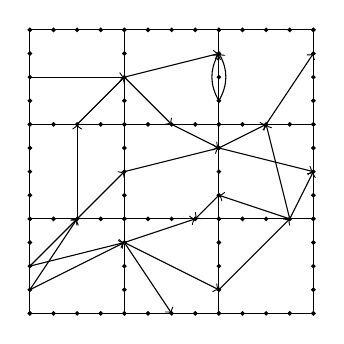
\begin{tikzpicture}[scale = 0.3]
\foreach \x in {0,...,12}{
\filldraw (\x,0) circle (2pt);
\filldraw (\x,4) circle (2pt);
\filldraw (\x,8) circle (2pt);
\filldraw (\x,12) circle (2pt);
}
\foreach \y in {0,...,12}
{
\filldraw (0,\y) circle (2pt);
\filldraw (4,\y) circle (2pt);
\filldraw (8,\y) circle (2pt);
\filldraw (12,\y) circle (2pt);
}
\draw[step=4] (0,0) grid (12,12);
\draw[->] (0,1) -- (4, 3);
\draw[->] (0,2) -- (2, 4);
\draw[->] (0,1) -- (2, 4);
\draw[->] (0,2) -- (4, 3);



\draw[->] (8,9) to[bend right] (8, 11);
\draw[->] (8,9) to[bend left] (8, 11);

\draw[->] (4,3) -- (7,4);
\draw[->] (4,3) -- (6,0);
\draw[->] (4,3) -- (8,1);
\draw[->] (8,1) -- (11,4);
\draw[->] (2,4) -- (2, 8);
\draw[->] (2,4) -- (4,6);
\draw[->] (4,6) -- (8,7);
\draw[->] (6,8) -- (8,7);
\draw[->] (8,5) -- (7,4);
\draw[->] (11,4) -- (8,5);
\draw[->] (11,4) -- (12,6);
\draw[->] (11,4) -- (10,8);
\draw[->] (8,7) -- (12, 6);
\draw[->] (8,7) -- (10,8);

\draw[->] (2,8) -- (4,10);
\draw[->] (0,10) -- (4,10);

\draw[->] (4,10) -- (6,8);
\draw[->] (4,10) -- (8,11);

\draw[->] (10, 8) -- (12,11);




\end{tikzpicture}

\end{subfigure}
%
\caption{A grid digraph $G$ divided into subgrids and its corresponding auxiliary digraph $\aux{G}$} %
\label{fig:auxG}

\end{figure}

%

%
\subsection{Properties of the auxiliary digraph} %
In the following definition, we give ordered labelling to the vertices of a block of the auxiliary 
 %
digraph. %
We define the labelling with respect to some vertex 
%
in the block.
\begin{definition}
\label{def:perm}
Let $G$ be a $m \times m$ grid 
 %
digraph, %
$\ell = \aux{G}[i,j]$ be a block of $\aux{G}$ and $v = (x, y)$ be a vertex in $\aux{G}[i,j]$. Let $t = m^{1-\alpha}$. We define a cyclic permutation $c_{\ell}$ on the vertex set of $\aux{G}[i,j]$ as follows:
\[ \ac{l}{}{v} = \begin{cases} (x +1 , y) &\text{ if } x < (i + 1)t \textup{ and } y = jt\\
(x, y +1)&\text{ if } x = (i + 1)t \textup{ and } y < (j + 1)t\\
(x-1, y) &\text{ if } x > it \textup{ and } y = (j + 1)t \\
(x, y -1)&\text{ if } x = it \textup{ and } y > jt \end{cases}\]
For any non-negative integer $r$, we define $c_{\ell}^r$ inductively as follows. For $r = 0$, $\ac{l}{r}{v} = v$ and otherwise we have $\ac{l}{r+1}{v} = \ac{l}{}{\ac{l}{r}{v}}$.
\end{definition}

 Note that the permutation $c_{\ell}$ can be seen as a counter-clockwise shift. Also note that for a block $\ell$ and vertices $v$ and $w$ in it, we can write $v$ as $\ac{l}{p}{w}$ where $p$ is smallest non-negative integer for which $\ac{l}{p}{w} = v$. Next we formalize what it means to say that two edges of the auxiliary %
digraph %
cross each other.

\begin{definition}
\label{def:cross}
Let $G$ be a grid 
 %
digraph %
and $\ell$ be a block of $\aux{G}$. For two distinct edges $e$ and $f$ in the block, such that $e = (v, \ac{l}{p}{v})$ and $f = (\ac{l}{q}{v}, \ac{l}{r}{v})$. We say that edges $e$ and $f$ cross each other if $\min(q, r) < p < \max(q, r)$.
\end{definition}

Note the definition of cross given above is symmetric. That is, if edges $e$ and $f$ cross each other then $f$ and $e$ must cross each other as well. For an edge $f = (\ac{l}{q}{v}, \ac{l}{r}{v})$, we define $\overleftarrow{f} = (\ac{l}{r}{v}, \ac{l}{q}{v})$ and call it the \emph{reverse} of $f$. We also note that if $e$ and $f$ cross each other, then $e$ and $\overleftarrow{f}$ also cross each other.

In \expref{Lemma}{lem:cross} we state an equivalent condition of the crossing of two edges. In \expref{Lemmas}{lem:psg} \expref{and}{lem:closer} we state some specific properties of the auxiliary 
 %
digraph %
that we use later.


\begin{lemma}
\label{lem:cross}
Let $G$ be a grid 
 %
digraph %
and $\ell$ be a block of $\aux{G}$. Let $w$ be an arbitrary vertex in the block $\ell$ and $e = (\ac{l}{p}{w}, \ac{l}{q}{w})$ and $f = (\ac{l}{r}{w}, \ac{l}{s}{w})$ be two distinct edges in $\ell$. Then $e$ and $f$ cross each other if and only if either of the following two conditions hold:
\begin{itemize}
\item $\min(p, q) < \min(r, s) < \max(p, q) < \max(r,s)$
\item $\min(r, s) < \min(p, q) < \max(r, s) < \max(p,q)$
\end{itemize}
\end{lemma}

\begin{proof}
We prove that if $\min(p, q) < \min(r, s) < \max(p, q) < \max(r,s)$ then $e$ and $f$ cross each other. We let $p < r < q < s$. Other cases can be proved by reversing appropriate edges. We thus have integers $r_1 = r - p$, $q_1 = q - p$ and $s_1 = s - p$. Clearly, $r_1 < q_1 < s_1$. Let $v = \ac{l}{p}{w}$. Thus we have $e = (v, \ac{l}{q}{w}) = (v, \ac{l}{q_1}{\ac{l}{p}{w}}) = (v, \ac{l}{q_1}{v})$ and $f = (\ac{l}{r}{w}, \ac{l}{s}{w}) = (\ac{l}{r_1}{\ac{l}{p}{w}}, \ac{l}{s_1}{\ac{l}{p}{w}}) = (\ac{l}{r_1}{v}, \ac{l}{s_1}{v})$
The proof for the second condition is similar.

Now, we prove that if $e = (\ac{l}{p}{w}, \ac{l}{q}{w})$ and $f = (\ac{l}{r}{w}, \ac{l}{s}{w})$ cross each other then either of the given two condition holds. We assume that $p$ is the smallest integer among $p$, $q$, $r$ and $s$. Other cases can be proved similarly. Now, let $v = \ac{l}{p}{w}$. We thus have integers $q_1 = q-p, r_1 = r-p$ and $s_1 = s-p$ such that $e = (v, \ac{l}{q_1}{v})$ and $f = (\ac{l}{r_1}{v}, \ac{l}{s_1}{v})$. Since $e$ and $f$ cross each other, we have $\min(r_1, s_1) < q_1 < \max(r_1, s_1)$. Thus $\min(r_1+p, s_1+p) < q_1+p < \max(r_1+p, s_1+p)$. It follows that $\min(r, s) < q < \max(r,s)$. Since we assumed $p$ to be smallest integer among $p$, $q$, $r$ and $s$; we have $\min(p, q) < \min(r, s) < \max(p, q) < \max(r,s)$, thus proving the lemma.
\end{proof}


We see that we can draw an auxiliary %
digraph %
on a plane such that the arcs corresponding to two of its edges intersect if and only if the corresponding edges cross each other. Henceforth, we will work with such a drawing.
\begin{definition}
Let $G$ be a grid %
digraph %
 and $\ell$ be a block of $\aux{G}$. For a vertex $v$ and edges $f$, $g$ such that $f = (\ac{l}{q}{v}, \ac{l}{r}{v})$ and $g = (\ac{l}{s}{v}, \ac{l}{t}{v})$, we say that $f$ is closer to $v$ than $g$ if $\min(q, r) < \min(s, t)$.

We say $f$ is \emph{closest} to $v$ if there exists no other edge $f'$ which is closer to $v$ than $f$.
\end{definition}

\begin{lemma}
\label{lem:psg}
Let $G$ be a grid %
digraph %
 and $e_1 = (u_1,v_1)$ and $e_2 = (u_2,v_2)$ be two edges in $\aux{G}$. If $e_1$ and $e_2$ cross each other, then $\aux{G}$ also contains the edges $(u_1, v_2)$ and $(u_2, v_1)$.
\end{lemma}
\begin{proof}
Let $e_1 = (v, \ac{l}{p}{v})$ and $e_2 = (\ac{l}{q}{v}, \ac{l}{r}{v})$ be two edges that cross each other in $\aux{G}$. Let $\ell$ be the block of $\aux{G}$ to which $e_1$ and $e_2$ belong. Consider the subgrid of $G$ which is solved to construct the block ${\ell}$. Since the edge $e_1$ exists in block ${\ell}$, there exists a path $P$ from $v$ to $\ac{l}{p}{v}$ in the underlying subgrid. This path $P$ divides the subgrid into two parts such that the vertices $\ac{l}{q}{v}$ and $\ac{l}{r}{v}$ belong to different parts of the subgrid. Thus, a path between $\ac{l}{q}{v}$ and $\ac{l}{r}{v}$ necessarly take a vertex of path $P$. Hence, there is a path from $v$ to $\ac{l}{r}{v}$ and a path from $\ac{l}{p}{v}$ to $\ac{l}{r}{v}$. Thus the lemma follows.
\end{proof}

\begin{figure}[ht]
\begin{center}
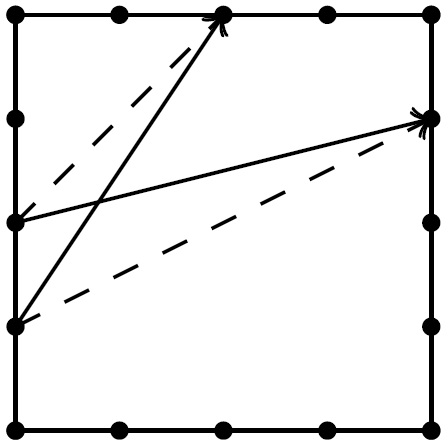
\includegraphics[width=0.3\textwidth]{solvedblock.jpg}
\hfill
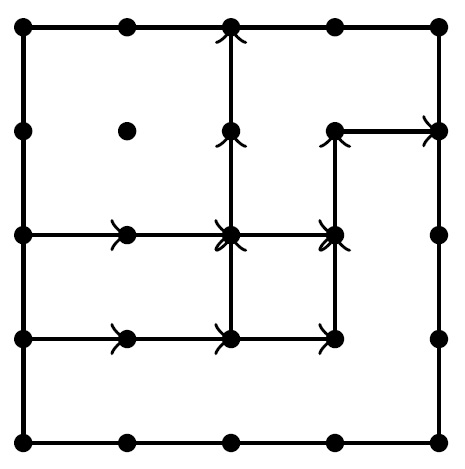
\includegraphics[width=0.3\textwidth]{block.jpg}

\end{center}
\caption{Edge crossings in an auxiliary grid. On the left, there is one block of the auxiliary %
digraph %
 that contains edges that cross. The dotted edges are the ones whose existence is made necessary by \expref{Lemma}{lem:psg}. On the right, a subgrid which results in the auxiliary block on the left.}
\end{figure}




\begin{lemma}
\label{lem:closer}
Let $G$ be a grid %
digraph %
 and $e_1 = (u_1,v_1)$ and $e_2 = (u_2,v_2)$ be two edges in $\aux{G}$. If $e_1$ and $e_2$ cross a certain edge $f = (x,y)$, and $e_1$ is $closer$ to $x$ than $e_2$, then the edge $(u_1, v_2)$ is also %
 in $\aux{G}$.
\end{lemma}

\begin{figure}
\centering
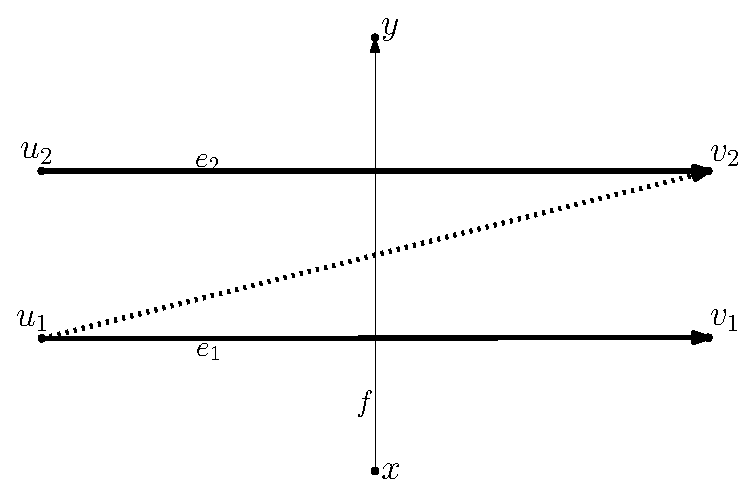
\includegraphics[width=0.9\textwidth]{observation.eps}

%
\caption{Illustration of \expref{Lemma}{lem:closer}}
\end{figure}

\begin{proof}
Let $f = (v, c_{\ell}^p(v))$, $e_1 = (c_{\ell}^q(v), c_{\ell}^r(v))$ and $e_2 = (c_{\ell}^s(v), c_{\ell}^t(v))$. If $c_{\ell}^q(v) = c_{\ell}^s(v)$ then the lemma trivially follows. Otherwise, we have two cases to consider:
\begin{description}
\item[Case 1 ($e_1$ crosses $e_2$):] In this case, we will have $(c_{\ell}^q(v), c_{\ell}^t(v))$ %
in $\aux{G}$ by \expref{Lemma}{lem:psg}.
\item[Case 2 ($e_1$ does not cross $e_2$):] In this case, we have $\min(q,r) < \min(s,t) < p < \max(s, t) < \max(q, r)$. Since $e_1$ crosses $f$, we have the edge $(c_{\ell}^q(v), c_{\ell}^p(v))$ in $\aux{G}$ by 
\expref{Lemma}{lem:psg}. This edge will cross $e_2$. Hence $(c_{\ell}^q(v), c_{\ell}^t(v))$ is %
 in $\aux{G}$.\qedhere
\end{description}
\end{proof}

%
\section{Pseudoseparators in a grid digraph}  %
\label{sec:pseudosep}
Imai et al. used a separator construction to solve the reachability problem in planar %
digraphs %
 \cite{Imai}. A separator is a set of vertices whose removal disconnects the graph into \emph{small components}. The class of grid %
digraphs %
%
is a subclass of planar %
digraphs. %
Grid graphs are known to have small separators. However, for a grid %
digraph %
 $G$, the %
underlying undirected graph of %
 $\aux{G}$ might not have a small separator.

An essential property of a separator is that, for any two vertices, a path between the vertices must contain a separator vertex if the vertices lie in two different components with respect to the separator. This property can then be used to design a divide and conquer %
algorithm for reachability where only separator vertices need to be marked and stored for traversal. \expref{Lemma}{lem:closer} allows us to use edges as well since, at most, one vertex on each side of an edge needs to be stored for traversal (the visited-vertex closest to the tail of the edge). Hence, we can use a slightly weaker structure in place of a separator. We construct a structure called pseudoseparator (see \expref{Definition}{def:psc}). It is essentially a set of vertices and edges that can be used to divide the %
digraph %
into components, such that a path from one component to another either takes a vertex of the pseudoseparator or crosses an edge of the pseudoseparator.

For a %
digraph %
$H = (V_1, E_1)$ given along with its drawing,
%
%
%
%
%
and a  %
sub-digraph %
$C = (V_2, E_2)$ of $H$, define the 
 %
digraph %
$\sep{H}{C} = (V_3, E_3)$ as $V_3 = V_1 \setminus V_2$ and $E_3 = E_1 \setminus \{e \in E_1 \mid \exists f \in E_2, e \textrm{ crosses } f\}$. We note that the %
digraph %
$H$ we will be working with throughout the article will be a  %
sub-digraph %
 of an auxiliary %
digraph. %
Hence it will always come with a drawing.

\begin{definition}
\label{def:psc}
Let $G$ be a grid %
digraph %
and $H$ be
%
%
an induced  %
 %
sub-digraph %
 of $\aux{G}$ with $h$ vertices. Let $f:\mathbb{N} \rightarrow \mathbb{N}$ be a function. A  %
sub-digraph %
 $C$ of $H$ is said to be an $f(h)$-$\psc$ of $\aux{G}$ if the size of every connected component in $\concom{\sep{H}{C}}$ is at most $f(h)$. The size of $C$ is the
%
%
%
number of vertices plus the number of edges of $C$.
\end{definition}

For
%
an induced%
  %
sub-digraph %
 $H$ of $\aux{G}$, an $f(h)$-$\psc$ is a  %
sub-digraph %
 $C$ of $H$ that has the property that, if we remove the vertices as well as all the edges that cross one of the edges of the $\psc$, the %
digraph %
 gets disconnected into small pieces. Moreover for every edge $e$ in $H$, if there exists distinct sets $U_1$ and $U_2$ in $\concom{\sep{H}{C}}$ such that one of the endpoints of $e$ is in $U_1$ and the other is in $U_2$, then there exists an edge $f$ in $C$ such that $e$ crosses $f$. Hence any path in $H$ that connects two vertices in different components of $H \diamond C$ must either contain a vertex of $C$ or must contain an edge that crosses an edge of $C$. We divide the %
digraph %
 using this $\psc$ and give an algorithm that recursively solves each  %
sub-digraph %
 and then combines their solution efficiently.
\subsection{Constructing a pseudoseparator}
Before working out the details below, we briefly comment on how to construct a $\psc$ of
%
an induced%
 %
sub-digraph %
 $H$ of $\aux{G}$. Ideally, we would have liked to have a set of cycles of $H$
%
%
%
%
%
%
such that the surfaces obtained by cutting along these cycles have %
a bounded number of vertices 
on it.%
However, such cycles might not exist. We instead pick a maximal subset of edges from $H$ so that no two edges cross (see \expref{Definition}{def:planar} and \expref{Lemma}{lem:planarG}). Then we triangulate the resulting graph. We show that this triangulated graph has the required cycles and can be found using Imai et al.'s separator algorithm. Call the triangulated graph %
$\trplanar{H}$ and the separator vertices as $S$. Since the cycles might have triangulated edges, we will add at most a constant number of vertices and edges from $H$ to \emph{shield} these triangulated edges. The vertex set of $\psc$ of $H$ will thus contain all the vertices of $S$ and at most four additional vertices for each edge of $\trplanar{H}[S]$ that is not %
 in $H$. The edge set of $\psc$ of $H$ will contain all the edges of $H$ which are also in $\trplanar{H}[S]$ and at most four additional edges for each edge of $\trplanar{H}[S]$ that is not %
 in $H$.

\begin{definition}
\label{def:planar}
Let $G$ be a grid %
digraph %
 and $H$ be
%
an induced  %
sub-digraph %
 of $\aux{G}$. We define $\mxplanar{H}$ as a  %
sub-digraph %
 of $H$. The vertex set of $\mxplanar{H}$ is same as that of $H$. For an edge $e \in H$, let ${\ell}$ be the block to which $e$ belongs and let $w$ be the lowest indexed vertex in that block. Then $e = (c^i_{\ell}(w), c^j_{\ell}(w))$ is in $\mxplanar{H}$ if there exists no other edge $f = (c^x_{\ell}(w), c^y_{\ell}(w))$ in $H$ such that $\min(x,y) < \min(i, j) < \max(x, y) < \max(i, j)$.
\end{definition}

In \expref{Lemma}{lem:planarG} we show that the %
digraph %
 $\mxplanar{H}$ is indeed planar. We also prove that the subset of edges that we have picked from $H$ is a maximal subset such that no two edges cross.

\begin{lemma}
\label{lem:planarG}
Let $G$ be a grid %
digraph %
and $H$ be
%
 an induced  %
sub-digraph %
 of $\aux{G}$. No two edges of $\mxplanar{H}$ cross each other. Moreover, for any edge $e$ in $H$ that is not in $\mxplanar{H}$, there exists another edge in $\mxplanar{H}$ that crosses $e$.
\end{lemma}
\begin{proof}
Let ${\ell}$ be a block of $\aux{G}$ and $w$ be the smallest index vertex of ${\ell}$. Let $e = (c^p_{\ell}(w), c^q_{\ell}(w))$ and $f = (c^r_{\ell}(w), c^s_{\ell}(w))$ be two edges of $H$ that cross. We have, by \expref{Lemma}{lem:cross}, that either $\min(p,q) < \min(r, s) < \max(p, q) < \max(r, s)$ or $\min(r,s) < \min(p, q) < \max(r, s) < \max(p, q)$. Hence, by our construction of $\mxplanar{H}$, atmost one of $e$ and $f$ belongs to it. Thus no two edges of $\mxplanar{H}$ %
 cross.

For the second part, we will prove by contradiction. Let us assume that there exists edges in $H$ which is not in $\mxplanar{H}$ and also not crossed by an edge in $\mxplanar{H}$. We pick edge $e = (c_{\ell}^p(w), c_{\ell}^q(w))$ from them such that $\min(p, q)$ of that edge is minimum. Since this edge is not %
 in $\mxplanar{H}$, we have by definition, an edge $f = (c_{\ell}^r(w), c_{\ell}^s(w))$ such that $\min(r,s) < \min(p, q) < \max(r, s) < \max(p, q)$. We pick the edge $f$ for which $\min(r,s)$ is minimum. Now, since this edge $f$ is not %
 in $\mxplanar{H}$, we have another edge $g = (c_{\ell}^i(w), c_{\ell}^j(w))$ in $\mxplanar{H}$ such that $\min(i,j) < \min(r, s) < \max(i, j) < \max(r, s)$. We pick $g$ such that $\min(i, j)$ is minimum and break ties by picking one whose $\max(i,j)$ is maximum. Now, we have the following cases:
\begin{description}
\item[Case 1 ($i < r < j < s$):] Note that $H$ is
%
an induced  %
sub-digraph %
 of $\aux{G}$. Thus, in this case, the edge $(c_{\ell}^i(w), c_{\ell}^s(w))$ will be %
 in $H$ due to \expref{Lemma}{lem:psg}. Since $i < p < s < q$, and $i< \min(r, s)$, this will contradict the way in which edge $f$ was chosen.
\item[Case 2 ($i < s < j < r$):] In this case, the edge $(c_{\ell}^r(w), c_{\ell}^j(w))$ will be %
 in $H$ due to \expref{Lemma}{lem:psg}. This edge will cross $e$ and hence not be %
 in $\mxplanar{H}$. Thus, we have an edge $g' = (c_{\ell}^{i'}(w), c_{\ell}^{j'}(w))$ in $\mxplanar{H}$ such that $\min(i', j') < j < \max(i',j') < r$. We will thus have two subcases.
\begin{description}
\item[Case 2a ($i < \min(i', j')$):] Here, we will have $i < \min(i', j') < j < \max(i', j')$. Hence this edge will cross $g$ giving a contradiction to the first part of this Lemma.
\item[Case 2b ($\min(i', j') \leq i$):] Here, this edge should have been chosen instead of $g$ contradicting our choice of $g$.
\end{description}
\end{description}
The analysis of two remaining cases where $j<s<i<r$ and $j < r < i < s$ are similar to Cases $1$ and $2$ respectively.
\end{proof}


\begin{definition}
Let $G$ be a grid %
digraph %
and $H$ be
%
an induced  %
sub-digraph %
 of $\aux{G}$. The graph $\trplanar{H}$ is formed by first running \expref{Algorithm}{alg:completeboundary} on $H$ and then triangulating the %
underlying undirected graph of the result%
\end{definition}


\begin{algorithm}
\LinesNumbered
\caption{Completing the boundary of $\mxplanar{H}$}
\label{alg:completeboundary}
\KwIn{ 
%
An %
induced  %
sub-digraph %
 $H$ of $\aux{G}$}
%

Output all the vertices of $H$\;
Output all the edges of $\mxplanar{H}$\;
\ForEach{block $\ell$ in $H$}{
	\ForEach{vertex $v$ of $H$ in $\ell$}{
		 $p \gets$ the smallest positive integer such that $c_{\ell}^p(v) \in V(H)$\;
		\If{$(v, c_{\ell}^p(v)) \notin E(\mxplanar{H})$}{
			Output the edge $(v, c_{\ell}^p(v))$\;
		} 
}
}
\end{algorithm}

Note that \expref{Algorithm}{alg:completeboundary} completes the boundary of each block. Thus, for any block, the vertices in its boundary form a simple cycle. Since the interiors of these cycles are disjoint, there is no edge that is drawn through more than one block in $\trplanar{H}$. Thus, each edge of $\trplanar{H}$ %
lies  %
either entirely inside \emph{one} of the blocks, or
%
lies  %
completely outside the whole $m \times m$ grid.

Now, for each of those edges added to $\trplanar{H}$ as part of triangulation that is inside one of the blocks, we define a set of at most four \emph{shield} edges.

\begin{definition}Let $G$ be a grid %
digraph %
 and $H$ be %
an induced  %
sub-digraph %
 of $\aux{G}$. Let $e = (v, w)$ be an edge in $\trplanar{H}$ such that $e$ is inside one of the blocks and $e$ is not %
 in $\mxplanar{H}$. Let $p$ and $q$ be integers such that $w = c_{\ell}^{p}(v)$ and $v = c_{\ell}^q(w)$.

\begin{itemize}
\item Let $p_1$ be the largest integer such that $p_1 < p$ and an edge $e_1$ with endpoints $v$ and $c_{\ell}^{p_1}(v)$ exists in $\mxplanar{H}$. $e_1$ is undefined if no such integer exists.
\item Let $p_2$ be the smallest integer such that $p_2 > p$ and an edge $e_2$ with endpoints $v$ and $c_{\ell}^{p_2}(v)$ exists in $\mxplanar{H}$. $e_2$ is undefined if no such integer exists.
\item Let $q_1$ be the largest integer such that $q_1 < q$ and an edge $e_3$ with endpoints $c_{\ell}^{q_1}(w)$ and $w$ exists in $\mxplanar{H}$. $e_3$ is undefined if no such integer exists.
\item Let $q_2$ be the smallest integer such that $q_2 > q$ and an edge $e_4$ with endpoints $c_{\ell}^{q_2}(w)$ and $w$ exists in $\mxplanar{H}$. $e_4$ is undefined if no such integer exists.
\end{itemize}
For $i = 1,2,3,4$, the edges $e_i$ which are defined above are called \emph{shield} edges of $e$.
\end{definition}

We will be using the following Lemma, which was proven by Imai et al., to help us in the construction of $\psc$.

\begin{lemma}\label{lem:seplemma}\cite{Imai}
For every $\beta > 0$, there exists a
%
polynomial-time   %
and $\tilde{O}(h^{1/2 + \beta/2})$-space %
algorithm that takes a $h$-vertex planar graph $P$ as input and outputs a set of vertices $S$, such that $|S|$ is $O(h^{1/2 + \beta/2})$ and removal of $S$ disconnects the graph into components of size $O(h^{1-\beta})$.
\end{lemma}

\expref{Algorithm}{alg:psepH} describes how to construct a  %
sub-digraph %
 of $H$ which we call $\psep(H)$. In \expref{Lemma}{lem:psep} we show that $\psep(H)$ is a $\psc$ of $H$.

\begin{algorithm}
\LinesNumbered
\caption{Construction of \psep(H)}
\label{alg:psepH}
\KwIn{%
An%
induced  %
sub-digraph %
 $H$ of $\aux{G}$ and a positive number $\beta$}
\KwOut{The %
digraph %
 \psep(H)}

Construct $\trplanar{H}$ from $H$\;
Find a set $S$ of vertices in $\trplanar{H}$ which divides it into components of size $O(n^{1-\beta})$ by applying \expref{Lemma}{lem:seplemma} \label{line:spacedom}\;
Output all the vertices of $S$\; 
Output those edges of %
$H$ which are also (in its undirected form) in $\trplanar{H}[S]$\;

\ForEach{edge $e = (v, w)$ of $\trplanar{H}$}{
\If{$e$ is \emph{inside} a block of $\trplanar{H}$ \textbf{and} $e \notin E(\mxplanar{H})$ \textbf{and} both endpoints of $e$ are in $S$}{
Output all the shield edges of $e$ along with their end vertices.
}
}
\end{algorithm}

\begin{lemma}\label{lem:psepcomplexity}
Let $G$ be a grid %
digraph %
, and $H$ be %
an%
 induced  %
sub-digraph %
 of $\aux{G}$. For every $\beta > 0$, there exists a polynomial-time %
and $\tilde{O}(h^{1/2 + \beta/2})$-space  %
algorithm that takes $H$ as input and outputs \psep(H).
\end{lemma}
\begin{proof}
  To prove this lemma, we analyse the space and time complexity of 
\expref{Algorithm}{alg:psepH}. We will first see that $\trplanar{H}$ %
is %
 constructed from $H$ in logspace. To see it, we first note that we can decide if an edge $e$ of $H$ belong to $\mxplanar{H}$ in logspace by checking if $e$ satisfies the condition required by \expref{Definition}{def:planar}. Next, the boundary of $\mxplanar{H}$ %
is %
 completed in logspace by using \expref{Algorithm}{alg:completeboundary}. Finally we triangulate the resultant graph in logspace: For every face $f$ in the resultant graph, we connect each vertex of $f$ to the lowest-indexed vertex of $f$. The space complexity of construction of \psep(H) is thus dominated by the space required by \expref{step}{line:spacedom} of \expref{Algorithm}{alg:psepH}. By \expref{Lemma}{lem:seplemma}, we know that this step requires $O(h^{1/2 + \beta/2})$ space. Hence, the space required by \expref{Algorithm}{alg:psepH} is $O(h^{1/2 + \beta/2})$. Each step of \expref{Algorithm}{alg:psepH} %
is %
 performed in polynomial time, hence the total time complexity is bounded by a polynomial.
\end{proof}

\begin{lemma}
\label{lem:psep}
Let $G$ be a grid %
digraph %
, and $H$ be %
an%
induced  %
sub-digraph %
 of $\aux{G}$. The %
digraph %
 $\psep(H)$ is a $h^{1-\beta}$-$\psc$ of $H$.
\end{lemma}
To prove \expref{Lemma}{lem:psep}, we first show a property of triangulated graphs that we use in our construction of $\psc$. We know that a simple cycle in a planar embedding of a planar graph divides the plane into two parts. We call these two parts the two \emph{sides} of the cycle.

\begin{lemma}
\label{lem:sepfamily}
Let $G$ be a triangulated planar graph, and $S$ be a subset of its vertices. For each pair of vertices $u, v$ belonging to different components of $G \setminus S$, a cycle in $G[S]$ exists, such that $u$ and $v$ belong to different sides of this cycle.
\end{lemma}

\begin{proof}
To prove the Lemma, we first need some terminology. We call a set of faces a \emph{region of edge-connected faces} if they induce a connected subgraph in the dual graph. We can orient the edges of an undirected planar simple cycle to make it a directed cycle. This can help us identify the two \emph{sides} of the cycle as \emph{interior} (left-side) and \emph{exterior} (right-side).

Let $C$ be a component of $G \setminus S$ and $S'$ be the set of vertices of $S$ adjacent to at least one of the vertices of $C$ in $G$. Let $F$ be the set of triangle faces of $G$ to which at least one vertex of $C$ belongs. Let $\tilde{G}$ be the dual graph of $G$ and $\tilde{G}[F]$ be the subgraph induced by $F$ on this dual graph.  %
%
%
%
%
%
%

%
We first observe that since we have started with a triangulated graph, the vertices of any face $f$ of $F$ will either belong to $C$ or $S'$. 

Let $f_1$ and $f_2$ be two arbitrary faces of $F$. We will first show that $F$ is a region of edge-connected faces by showing that there exists a path between $f_1$ and $f_2$ in $\tilde{G}[F]$. Let $v_1$ be a vertex of $C$ which belongs to $f_1$. Similarly, let $v_2$ be a vertex of $C$ which belongs to $f_2$. Let the length of shortest path between $v_1$ and $v_2$ in $G \setminus S$ be $k$. We prove our claim by induction on $k$. If $k = 0$, then $v_1 = v_2$. We know that the set of faces that share a vertex induce a connected subgraph in the dual graph, hence our claim holds for $k=0$.
Now, we assume that our claim holds for path length $k = \ell-1$. To prove that our claim holds for $k= \ell$, let $(v_3, v_2)$ be the last edge in the shortest path from $v_1$ to $v_2$. Let $f_3$ be a face with both $v_3$ and $v_2$ in its boundary. Since the length of shortest path from $v_1$ to $v_3$ is $\ell-1$, by induction hypothesis, there exists a path between $f_1$ and $f_3$ in $\tilde{G}[F]$. Since $f_3$ and $f_2$ share the vertex $v_2$, there is a path between $f_3$ and $f_2$ in $\tilde{G}[F]$. Combining these two paths, we get a path between $f_1$ and $f_2$ in $\tilde{G}[F]$ which proves our claim.

Miller proved that the boundary of a region of edge-connected faces is a set of edge-disjoint \emph{simple} cycles which can be oriented such that they have disjoint exteriors \cite{Miller}. We claim that all the vertices of any boundary cycle of $F$ are contained in $S'$. We prove this claim by contradiction. Let us assume that $v$ is a vertex in a boundary cycle of $F$ that is not %
 in $S'$. In this case, $v$ belongs to $C$. Consider an edge $(v,w)$ of the boundary cycle. Let $f_a$ and $f_b$ be the two faces that shares the edge $(v,w)$. Let $v_a$ and $v_b$ be the third vertex of $f_a$ and $f_b$ respectively. Since $v_a$, $v_b$ and $w$ are all connected to $v$, they are %
 in either $S'$ or $C$. Thus both $f_a$ and $f_b$ are in $F$. However, this contradicts that $(v,w)$ is at boundary of $F$. 

Thus, we have proved that the vertices of a connected component of $G\setminus S$ are contained inside a set of edge-disjoint simple cycles with disjoint exteriors. The vertices of all such cycles are contained in $S$. Hence the lemma follows.
\end{proof}

\begin{proof}[Proof of \expref{Lemma}{lem:psep}]
Let $C = \psep(H)$. Let $S$ be the set of vertices obtained from $\trplanar{H}$ by using \expref{Lemma}{lem:seplemma}. We claim that if any two vertices $u$ and $v$ belong to different connected components of $\trplanar{H} \setminus S$, then it belongs to different components of $\concom{\sep{H}{C}}$. We prove this by contradiction. Let us assume that it is not true. Then there is an edge $e$ in $H$ and two distinct sets $U_1$ and $U_2$ of $\concom{\trplanar{H}\setminus S}$ such that one of the end point of $e$ is in $U_1$, the other is in $U_2$ and $e$ does not cross any of the edges of $\psep(H)$. Without loss of generality, let $e = (v, c_{\ell}^p(v))$, for some block $\ell$, where $v \in U_1$ and $c_{\ell}^p(v)$ is not in $U_1$ (we pick the edge $e$ such that $p$ is minimum for any choice of $v$). Due to \expref{Lemma}{lem:sepfamily}, it follows that there exists an edge $f$ in $\trplanar{H}[S]$ such that $f = ((c_{\ell}^q(v)), c_{\ell}^r(v))$ and that $e$ crosses $f$. This edge $f$ is a triangulation edge, for otherwise it is also %
 in \psep(H) giving us a contradiction. We orient the triangulation edge so that $q < p < r$. Now, since $e$ is not %
 in $\mxplanar{H}$, by \expref{Lemma}{lem:planarG} there exists at least one edge that crosses it and is %
 in $\mxplanar{H}$. Let $g = (c_{\ell}^s(v), c_{\ell}^t(v))$ be one such edge such that $t - s$ is maximum\footnote{We note that we do \emph{not} consider the \emph{absolute} value of the $t-s$, rather we consider the actual value. $t-s$ can hence be negative for an edge.} We thus have the following cases:
\begin{description}
\item[Case 1 ($s<q<p<r<t$):] In this case, since $g$ crosses $e$, by
\expref{Lemma}{lem:psg}, we have that the edge $e' = (c_{\ell}^s(v), c_{\ell}^p(v))$ is also %
 in $H$. $e'$ also crosses $f$. Since $p-s < p$, existence of $e'$ contradicts our choice of $e$.
\item[Case 2 ($q<t<p<s<r$):] In this case, since $g$ crosses $e$, by 
\expref{Lemma}{lem:psg}, we have that the edge $e' = (v, c_{\ell}^t(v))$ is also %
 in $H$. $e'$ also crosses $f$. Since $t < p$, existence of $e'$ contradicts our choice of $e$.
\item[Case 3 ($t<q<p<r<s$):] In this case, the edge $e' = (c_{\ell}^{s}(v), c_{\ell}^p(v))$ will also be %
 in $H$. $e'$ will cross $f$ and hence will not be %
 in $\mxplanar{H}$. By \expref{Lemma}{lem:planarG}, there exists an edge $g' = (c_{\ell}^{s'}(v), c_{\ell}^{t'}(v))$ in $\mxplanar{H}$ that crosses $e'$. Since both $g'$ and $g$ are %
 in $\mxplanar{H}$, these edges %
do not %
cross each other. 

Using the fact that $g'$ crosses $e'$ and $g'$ does not cross $g$, we get the following:

\[t \leq \min(s',t') < p < \max(s', t') < s\]

Consequently, $t'-s' > t-s$ and $g'$ crosses $e$. This contradicts our choice of $g$.


\item[Case 4 ($q<s<p<t<r$):] In this case, since $g$ crosses $e$, by
\expref{Lemma}{lem:psg}, we have that the edge $e' = (v, c_{\ell}^t(v))$ is %
 in $H$. $e'$ also crosses $f$ and hence $e'$ was not %
 in $\mxplanar{H}$. Thus there will exist an edge in $\mxplanar{H}$ which crosses $e'$ by \expref{Lemma}{lem:planarG}. Let $g' = (c_{\ell}^{s'}(v), c_{\ell}^{t'}(v))$ be the edge in $\mxplanar{H}$ that crosses $e'$ such that $t'-s'$ is maximum. We have the following subcases:
\begin{description}
\item[Case 4a ($s'<q<t<r<t'$):]In this case, since $g'$ crosses $e$, by \expref{Lemma}{lem:psg}, we have that the edge $e'' = (c_{\ell}^{s'}(v), c_{\ell}^p(v))$ is also %
 in $H$. $e''$ also crosses $f$. Since $p-s' < p$, existence of $e''$ contradicts our choice of $e$.
\item[Case 4b ($q<t'<t<s'<r$):] In this case, we see that since $g$ and $g'$ are both %
 in $\mxplanar{H}$, they
 %
do not %
cross each other. Therefore. $t' \leq s$ and consequently $t' < p$. Thus, $g'$ crosses $e$ and by \expref{Lemma}{lem:psg}, the edge $e'' = (v, c_{\ell}^{t'}(v))$ is also %
 in $H$. $e''$ also crosses $f$. Since $t' < p$, existence of $e''$ contradicts our choice of $e$.
\item[Case 4c ($t'<q<t<r<s'$):] In this case, the edge $e'' = (c_{\ell}^{s'}(v), c_{\ell}^t(v))$ will also be %
 in $H$. $e''$ will cross $f$ and hence will not be %
 in $\mxplanar{H}$. By \expref{Lemma}{lem:planarG}, there exists an edge $g'' = (c_{\ell}^{s''}(v), c_{\ell}^{t''}(v))$ in $\mxplanar{H}$ that crosses $e''$. Since $g''$, $g'$ and $g$ are all %
 in $\mxplanar{H}$, these edges 
 %
do not %
cross each other. 

Using the fact that $g''$ crosses $e''$, $g''$ does not cross $g'$ and $g''$ does not cross $g$; we get the following:

\[t' \leq \min(s'',t'') <s< t < \max(s'', t'') < s'\]

Consequently, $t''-s'' > t'-s'$ and $g''$ crosses $e'$. This contradicts our choice of $g'$.

\item[Case 4d ($q<s'<t<t'<r$):] In this case, we see that since $g$ and $g'$ are both %
 in $\mxplanar{H}$, they
 %
do not %
cross each other. Therefore $s' \leq s$ and consequently $s' < p$. Thus, $g'$ crosses $e$ and $t' - s' > t-s$. This contradicts our choice of $g$.

\end{description}
\end{description}
In other cases, if $g$ is picked such that one of its vertices is common with $f$, then $e$ will cross a $shield$ edge of $f$, giving a contradiction. If $g$ is picked such that $g$ cross $f$, then it contradicts the fact that both of them are %
 in $\trplanar{H}$, which is a planar %
digraph %
.
\end{proof}
Summarizing \expref{Lemmas}{lem:psepcomplexity} \expref{and}{lem:psep} we have \expref{Theorem}{thm:constructpsc}.
\begin{theorem} \label{thm:constructpsc}
Let $G$ be a grid %
digraph %
 and $H$ be %
an%
induced subgraph of $\aux{G}$ with $h$ vertices. For any constant $\beta > 0$, there exists an $\tilde{O}(h^{1/2 + \beta/2})$-space and polynomial-time %
algorithm that takes $H$ as input and outputs an $h^{1-\beta}$-$\psc$ of size $O(h^{1/2 + \beta/2})$.
\end{theorem}

%
\section{Algorithm to solve reachability in the auxiliary %
digraph %
}   %
\label{sec:auxreach}
	\begin{figure}
		\centering
		\begin{subfigure}{0.4\textwidth}
			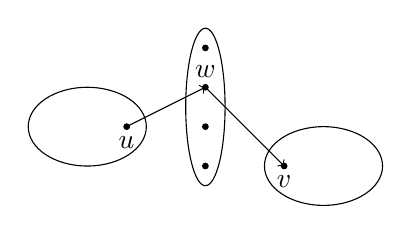
\begin{tikzpicture}[scale = 0.5]
			
			\filldraw (-1,2) circle (2pt) node[below] {$u$};    
			\filldraw (1,1) circle (2pt);    
			\filldraw (1,2) circle (2pt);    
			\filldraw (1,3) circle (2pt) node[above] {$w$};    
			\filldraw (1,4) circle (2pt);
			\filldraw (3,1) circle (2pt) node[below] {$v$};	
			
			\draw (-2,2) circle [x radius=1.5cm, y radius=10mm];		
			\draw[->] (-1,2) -- (1,3);
			
			\draw (4,1) circle [x radius=1.5cm, y radius=10mm];	
			\draw[->] (1,3) -- (3,1);
			
			\draw (1,2.5) circle [x radius=0.5cm, y radius=20mm];		
			
			
			\end{tikzpicture}
			
			\caption{\scriptsize The $s$-$t$ path takes a vertex of the separator}
			\label{fig:viaseparator}
			
		\end{subfigure}
	\hfill
		\begin{subfigure}{0.4\textwidth}
			\centering
			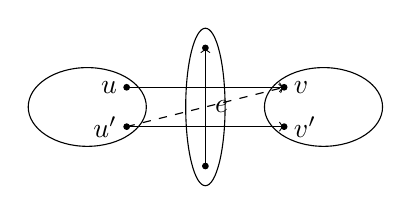
\begin{tikzpicture}[scale = 0.5]
			
			\filldraw (-1,2) circle (2pt) node[left] {$u'$};    
			\filldraw (1,1) circle (2pt) ;
			\filldraw (1,4) circle (2pt) ;
			\filldraw (3,2) circle (2pt) node[right] {$v'$};			
			
			\filldraw (-1,3) circle (2pt) node[left] {$u$};			
			\filldraw (3,3) circle (2pt) node[right] {$v$};			
			
			\draw[->] (-1,2) -- (3,2);
			
			\draw (-2,2.5) circle [x radius=1.5cm, y radius=10mm];
			\draw (1,2.5) circle [x radius=0.5cm, y radius=20mm];	
			\draw (4,2.5) circle [x radius=1.5cm, y radius=10mm];		
			
			
			\draw[->] (-1,3) -- (3,3);
			\draw[->] (1,1) --node[right] {$e$} (1,4) ;
			\draw[dashed, ->] (-1, 2) -- (3,3);  
			
			
			\end{tikzpicture}
			
			\caption{\scriptsize The $s$-$t$ path crosses an edge of the separator}
			\label{fig:viaedgecrossing}
		\end{subfigure}
		
		\caption{ }
		
	\end{figure}
In this section, we discuss the grid %
digraph %
 reachability algorithm. Let $G$ be a grid %
digraph %
 having $\widetilde{n}$ vertices. By induction, we assume that we have access to %
an %
induced subgraph $H$ of $\aux{G}$, containing $h$ vertices. Below we describe a recursive procedure $\auxreach{H}{x}{y}$ that outputs \textsf{true} if there is a path from $x$ to $y$ in $H$ and outputs \textsf{false} otherwise.

\subsection{Description of the algorithm \textsf{AuxReach}}

First we construct a $h^{1-\beta}$-$\psc$ $C$ of $H$, using \expref{Theorem}{thm:constructpsc}. We also ensure that $x$ and $y$ are part of $C$ (if not then we add them). Let $I_1, I_2, \ldots, I_{\ell}$ be the connected components of $\sep{H}{C}$.

We maintain an array called \textsf{visited} of size $|C|$ to mark vertices or edges of the $\psc$ $C$. Each cell of \textsf{visited} corresponds to a distinct vertex or edge of $C$. For a vertex $v$ in $C$, we set $\textsf{visited}[v] := 1$ if there is a path from $x$ to $v$ in $H$, else it is set to 0. For an edge $e = (u,v)$ in $C$, we set $\textsf{visited}[e] := u'$ if (i) there is an edge $f = (u',v')$ that crosses $e$, (ii) there is a path from $x$ to $u'$ in $H$ and (iii) $f$ is the closest such edge to $u$. Else $\textsf{visited}[e]$ is set to \textsf{NULL}. Initially, for all vertex $v \in C$, $\textsf{visited}[v] := 0$ and for all edges $e \in C$, $\textsf{visited}[e] := \textsf{NULL}$. We say that a vertex $v$ is \emph{marked} if either $\textsf{visited}[v] = 1$ or $\textsf{visited}[e] = v$ for some edge $e$.

First set $\textsf{visited}[x]:=1$. We then perform an outer loop with $h$ iterations and in each iteration update certain entries of the array $\textsf{visited}$ as follows. For every vertex $v \in C$, the algorithm sets $\textsf{visited}[v]:=1$ if there is a path from a marked vertex to $v$ such that the internal vertices of that path all belong to only one component $I_i$. Similarly, for each edge $e = (u,v)$ of $C$, the algorithm sets $\textsf{visited}[e]:=u'$ if (i) there exists an edge $f = (u',v')$ which crosses $e$, (ii) there is a path from a marked vertex to $u'$ such that the internal vertices of that path all belong to only one component $I_i$ and, (iii) $f$ is the closest such edge to $u$. Finally we output \textsf{true} if $\textsf{visited}[y] = 1$ else output \textsf{false}. We use the procedure \textsf{AuxReach} recursively to check if there is a path between two vertices in a single connected component of $\sep{H}{C}$. A formal description of \textsf{AuxReach} is given in \expref{Algorithm}{alg:psgreach}.
\subsection{Proof of correctness of \textsf{AuxReach}}

Let $P$ be a path from $x$ to $y$ in $H$. Suppose $P$ passes through the components $I_{\sigma_1}, I_{\sigma_2}, \ldots, I_{\sigma_L}$ in this order. The length of this sequence %
is %
 at most $\lvert H \rvert$. As the path leaves the component $I_{\sigma_j}$ and goes into $I_{\sigma_{j+1}}$, it can do in the following two ways only:
\begin{enumerate}
\item The path exits $I_{\sigma_j}$ through a vertex $w$ of $\psc$ as shown in \expref{Figure}{fig:viaseparator}. In this case, \expref{Algorithm}{alg:psgreach} %
marks  %
the vertex $w$.
\item The path exits $I_{\sigma_j}$ through an edge $(u, v)$ whose other endpoint is in $I_{\sigma_{j+1}}$. By \expref{Lemma}{lem:closer}, this edge will cross an edge $e = (x',y')$ of the $\psc$. In this case, \expref{Algorithm}{alg:psgreach} %
marks  %
the vertex $u'$, such that there is an edge $(u', v')$ that crosses $e$ as well and $(u',v')$ is closer than $(u,v)$ to $x'$ and there is a path in $I_{\sigma_j}$ from a marked vertex to $u'$. By \expref{Lemma}{lem:closer}, the edge $(u', v)$ %
is  %
%
 in $H$ as well.
\end{enumerate}
\begin{algorithm}
\LinesNumbered
\caption{$\auxreach{H}{s}{t}$}
\label{alg:psgreach}
\KwIn{%
An %
induced subgraph $H$ of $\aux{G}$ and two vertices $x$ and $y$ in $H$ (let $G$ be an $m \times m$ grid %
digraph %
 and $h = |V(H)|$)}
\KwOut{\textsf{true} if there is a path from $x$ to $y$ in $H$ and \textsf{false} otherwise}

\lIf(\tcc*[f]{$m$ is a global variable where $G$ is an $m \times m$ grid %
digraph %
}){$h \leq m^{1/8} $}{
Use DFS to solve the problem}  \label{line:line1}
\Else{
Compute a $h^{1-\beta}$-$\psc$ $C$ of $H$ using \expref{Theorem}{thm:constructpsc}\; \label{line:calcpsep}
$C \gets C \cup \{x,y\}$\;
\lForEach{edge $e$ in $C$}{$\textsf{visited}[e] \gets \textsf{NULL}$}
\lForEach{vertex $v$ in $C$}{$\textsf{visited}[v] \gets 0$}
$\textsf{visited}[x] \gets 1$\;

\For{$i = 1$ to $\lvert H \rvert$}{ \label{alg:forloop}
\ForEach{edge $e = (u,v) \in C$}{



$\textsf{closestedge} \gets \textsf{NULL}$\;
\ForEach{marked vertex $w$}{
	\ForEach{$U \in \concom{\sep{H}{C}}$}{
		\ForEach{edge $f = (u',v')$ such that $f$ crosses $e$}{
			\If{$\auxreach{H[U \cup \{w, u' \}]}{w}{u'} = \textsf{true}$}{
				\If{$\textsf{closestedge} =\textsf{NULL}$  \textbf{or} $f$ is closer to $e$ than $\textsf{closestedge}$}{
					$\textsf{visited}[e] \gets u'$\;\label{line:recur1}
					$\textsf{closestedge} \gets f$\;
				}
			}
		}
	}
}
}
\ForEach{vertex $v \in C$}{
\If{$\exists w \exists U$ such that $w $ is 
%
%
a marked vertex\ {\bf and}\ $U \in \concom{\sep{H}{C}}$\
{\bf and}\ $\auxreach{H[U \cup \{w, v \}]}{w}{v} = \textsf{true}$))}{  
$\textsf{visited}[v] \gets 1$\; \label{line:recur2}}
}
}
\lIf{$\textsf{visited}[y] =1$}{\Return \textsf{true}}
\lElse{\Return \textsf{false}}
}
\end{algorithm}
Thus after the $j$-th iteration, \textsf{AuxReach}
%
traverses  %
the fragment of the path in the component $I_{\sigma_j}$ and either
%
marks  %
its endpoint or a vertex which is closer to the edge $e$ of $C$ which the path crosses. Finally, $y$ %
is  %
marked after $L$ iterations if and only if there is a path from $x$ to $y$ in $H$. We give a formal proof of correctness in \expref{Lemma}{lem:algo_correctness}. For a path $P = (u_1, u_2, \ldots u_t)$, we define $\tail{P} := u_1$ and $\head{P} := u_t$.

\begin{lemma}
\label{lem:algo_correctness}
Let $G$ be a grid %
digraph %
 and $H$ be %
an%
induced subgraph of $\aux{G}$. Then for any two vertices $x,y$ in $H$, there is a path from $x$ to $y$ in $H$ if and only if $\auxreach{H}{x}{y}$ returns \textsf{true}.
\end{lemma}
\begin{proof}
Firstly observe that, if a vertex is marked, then there is a path from some other marked vertex to that vertex in $H$. Hence if there is no path from $x$ to $y$ then $y$ is never marked by \textsf{AuxReach} and hence \textsf{AuxReach} returns \textsf{false}.

Now let $P$ be a path from $x$ to $y$ in $H$. We divide the path into subpaths $P_1, P_2 , \ldots , P_{\ell}$, such that for each $i$, all vertices of $P_i$ belong to $U \cup V(C)$ for some connected component $U$ in $\concom{\sep{H}{C}}$ and either (i) $\head{P_i} = \tail{P_{i+1}}$, or (ii) $e_i = (\head{P_i} , \tail{P_{i+1}})$ is an edge that crosses some edge $f_i \in C$. By \expref{Definition}{def:psc}, we have that if condition (i) is true then $\head{P_i}$ is a vertex in $C$, and if condition (ii) is true then $\head{P_i}$ and $\tail{P_{i+1}}$ belong to two different components of $\concom{\sep{H}{C}}$ and $e_i$ is the edge between them.

We claim that after $i$-th iteration of loop in \expref{Line}{alg:forloop} of \expref{Algorithm}{alg:psgreach}, either of the following two statements hold:
\begin{enumerate}
\item $\head{P_i}$ is a vertex in $C$ and $\textsf{visited}[\head{P_i}] = 1$.
\item There exists an edge $f_i = (u_i, v_i)$ of $C$ such that the edge $e_i = (\head{P_i}, \tail{P_{i+1}})$ crosses $f_i$ and there is an edge $g_i = (u_i',v_i')$ which crosses $f_i$ as well, such that $g_i$ is closer to $u_i$ than $e_i$ and $\textsf{visited}[f_i] = u_i'$.
\end{enumerate}
We prove the claim by induction. The base case holds since $x$ is marked at the beginning. We assume that the claim is true after the $(i-1)$-th iteration. We have that $P_i$ belongs to $U \cup V(C)$ for some connected component $U$ in $\concom{\sep{H}{C}}$.
\begin{description}
\item[Case 1 ($\head{P_{i-1}} = \tail{P_{i}} = w$(say)):] By induction hypothesis $w$ was marked after the $(i-1)$-th iteration. If $\head{P_i}$ is a vertex in $C$ then it will be marked after the $i$-th iteration in \expref{Line}{line:recur2}. On the other hand if $e_i = (\head{P_i} , \tail{P_{i+1}})$ is an edge that crosses some edge $f_i = (u_i,v_i) \in C$ then in the $i$-th iteration in \expref{Line}{line:recur1}, the algorithm marks a vertex $u_i'$ such that, $g_i = (u_i',v_i')$ is the closest edge to $u_i$ that crosses $f_i$ and there is a path from $w$ to $u_i'$.

\item[Case 2 ($e_{i-1} = (\head{P_{i-1}} , \tail{P_{i}})$ crosses some edge $f_{i-1} = (u_{i-1},v_{i-1}) \in C$):] By induction hypothesis, there is an edge $g_{i-1} = (u_{i-1}',v_{i-1}')$ which crosses $f_{i-1}$ as well, such that $g_{i-1}$ is closer to $u_{i-1}$ than $e_{i-1}$ and $\textsf{visited}[f_{i-1}] = u_{i-1}'$. By \expref{Lemma}{lem:closer} there is an edge in $H$ between $u_{i-1}'$ and $\tail{P_{i}}$ as well.
Now if $\head{P_i}$ is a vertex in $C$ then it will be marked after the $i$-th iteration in \expref{Line}{line:recur2} by querying the %
digraph %
 $H[U \cup \{u_{i-1}', \head{P_i}\}]$. On the other hand if $e_i = (\head{P_i} , \tail{P_{i+1}})$ is an edge that crosses some edge $f_i = (u_i,v_i) \in C$ then in the $i$-th iteration in \expref{Line}{line:recur1}, \textsf{AuxReach} queries the %
digraph %
 $H[U \cup \{u_{i-1}', u_i'\}]$ and marks a vertex $u_i'$ such that, $g_i = (u_i',v_i')$ is the closest edge to $u_i$ that crosses $f_i$ and there is a path from $u_{i-1}'$ to $u_i'$.\qedhere\end{description}\end{proof}

Our subroutine %
%
solves  %
reachability in a subgraph $H$ (having size $h$) of $\aux{G}$. We do not explicitly store a component of $\concom{\sep{H}{C}}$, since it might be too large. Instead, we identify a component with the lowest indexed vertex %
 in it and use Reingold's algorithm on $\sep{H}{C}$ to determine if a vertex is %
 in that component. We require $\widetilde{O}(h^{1/2 + \beta/2})$ space to compute a $h^{1-\beta}$-$\psc$ by \expref{Theorem}{thm:constructpsc}. We can potentially mark all the vertices of the $\psc$ and for each edge of
the  %
$\psc$ we mark at most one additional vertex. Since the size of
the  %
$\psc$ is at most $O(h^{1/2 + \beta/2})$, we require $\widetilde{O}(h^{1/2 + \beta/2})$ space. The algorithm recurses on a %
digraph %
 with $h^{1 - \beta}$ vertices.  %
Since we stop the recursion when $h \le m^{1/8}$
(\expref{Line}{line:line1} of \expref{Algorithm}{alg:psgreach}), %
the depth of the recursion is at most
%
$\lceil -3/\log(1-\beta)\rceil$,  %
which is a constant.

Since the %
digraph %
 $H$ is given implicitly in our algorithm, an additional polynomial overhead is involved in obtaining its vertices and edges. However, the total time complexity %
remains  %
a polynomial in the number of vertices since the recursion depth is constant.

\begin{lemma}
Let $G$ be an $m \times m$ grid %
digraph %
 and $H$ be%
an%
induced subgraph of $\aux{G}$ with $h$ vertices. For every $\beta > 0$, \textsf{AuxReach} runs in $\widetilde{O}({h}^{1/2 + \beta/2})$ space and polynomial time.
\end{lemma}
\begin{proof}
  Since the size of a component $U$ in $\concom{\sep{H}{C}}$ might be too large, we will not explicitly store it. Instead we identify a component by the lowest index vertex %
 in it and use Reingold's algorithm on $\sep{H}{C}$ to determine if a vertex is %
 in $U$. Let $S(m,h)$ and $T(m,h)$ denote the space and time complexity functions respectively of \textsf{AuxReach}, where $G$ is an $m \times m$ grid %
digraph %
 and $h$ is the number of vertices in the %
digraph %
 $H$. As noted earlier the depth of the recursion is at most 
%
$d:= \lceil -3/\log(1-\beta)\rceil$. %

Consider $S(m,h)$ for any $h > m^{1/8}$. By \expref{Theorem}{thm:constructpsc}, we require $\widetilde{O}(h^{1/2 + \beta/2})$ space to execute \expref{Line}{line:calcpsep}. We can potentially mark all the vertices of $C$ and for each edge $e$ of $C$ we store at most one additional vertex in $\textsf{visited}[e]$. Since the size of $C$ is at most $O(h^{1/2 + \beta/2})$, we require $\widetilde{O}(h^{1/2 + \beta/2})$ space to store $C$. By induction, a call to \textsf{AuxReach} in \expref{line}{line:recur1} \expref{and}{line:recur2} requires $S(m, h^{1 - \beta})$ space which can be subsequently reused. Hence the space complexity satisfies the following recurrence. Then,
\[S(m,h) =
\begin{cases}
S(m, h^{1 - \beta}) + \widetilde{O}(h^{1/2 + \beta/2}) & h > m^{1/8}\\
\widetilde{O}(h) & \textrm{otherwise}.
\end{cases}\]
Solving we get $S(m,h) = \widetilde{O}(h^{1/2 + \beta/2} + m^{1/4})$.

Next we measure the time complexity of \textsf{AuxReach}. Consider the case when $h > m^{1/8}$. The total number of steps in \textsf{AuxReach} is some polynomial in $h$, say $p$. Moreover \textsf{AuxReach} makes $q$ calls to \textsf{AuxReach}, where $q$ is some other polynomial in $h$. Hence $q(h) \leq p(h)$. Then,
\[T(m,h) =
\begin{cases}
q\cdot T(h^{1 - \beta}) + p & h > m^{1/8} \\
O(h) & \textrm{otherwise}.
\end{cases} \]
Solving the above recurrence we get $T(m,h) = O(p\cdot q^d + m^{1/4}) = O(p^{2d} + m^{1/4})$.
\end{proof}

\section{Solving grid %
digraph %
}
\label{sec:final}
Let $G$ be an $m \times m$ grid %
digraph %
. As mentioned in the introduction, our objective is to run the \expref{algorithm}{alg:psgreach} on the %
digraph %
 $\aux{G}$. Consider two vertices $x$ and $y$ of $\aux{G}$. Note that, by definition, $y$ is reachable from $x$ in $\aux{G}$ if and only if $y$ is reachable from $x$ in $G$. Hence it is sufficient to work with the %
digraph %
 $\aux{G}$. However, we do not have explicit access to the edges of $\aux{G}$. Note that we can obtain the edges of $\aux{G}$ by solving the corresponding subgrid of $G$ to which that edge belongs. If the subgrid is small enough, then we use a standard linear %
space-traversal  %
algorithm. Otherwise, we use our algorithm recursively on the subgrid. \expref{Algorithm}{alg:gridreach} outlines this method.
\begin{algorithm}
\caption{\textsf{GridReach}$(\widehat{G}, \widehat{s}, \widehat{t}, m)$}
\label{alg:gridreach}
\KwIn{A grid %
digraph %
 $\widehat{G}$ and two vertices $\widehat{s}$, $\widehat{t}$ of $\widehat{G}$ and a positive integer $m$}
\KwOut{\textsf{true} if there is a path from $s$ to $t$ in $G$ and \textsf{false} otherwise}
\If{$\widehat G$ is smaller than $m^{1/8} \times m^{1/8}$ grid}{
Use Depth-First Search to solve the problem\;
}
\Else
{
Use \textsf{ImplicitAuxReach}$(\aux{G}, \widehat{s}, \widehat{t})$ to solve the problem\;
\tcc*[f]{\textsf{ImplicitAuxReach} executes the same way as \textsf{AuxReach} except for the case when it queries an edge $(u, v)$ in a block $B$ of $\aux{G}$. In this case, the query is answered by calling \textsf{GridReach}$(B, u, v, m)$ where $B$ is the subgrid in which edge $(u,v)$ might belong.}
}
\end{algorithm}

Consider an $\widehat{m} \times \widehat{m}$ grid %
digraph %
 $\widehat{G}$. Let $S(\widehat{m})$ be the space complexity and $T(\widehat{m})$ be the time complexity of executing \textsf{GridReach} on $\widehat{G}$. Note that the size of $\aux{\widehat{G}}$ is at most $\widehat{m}^{1 + \alpha}$. For $\widehat{m} > m^{1/8}$, the space required to solve the grid %
digraph %

%
is   %
$S(\widehat{m}) = S(\widehat{m}^{1-\alpha}) + \widetilde{O}((\widehat{m}^{1+\alpha})^{1/2 + \beta/2})$. This is because, a query whether $(u,v) \in \widehat{G}$%
invokes  %
a recursion which %
requires  %
$S(\widehat{m}^{1-\alpha})$ space and the main computation of \textsf{ImplicitAuxReach} %
can  %
be done using $\widetilde{O}((\widehat{m}^{1+\alpha})^{1/2 + \beta/2})$ space. Hence we get the following recurrence for space complexity.
\[S(\widehat{m}) =
\begin{cases}
S(\widehat{m}^{1 - \alpha}) + \widetilde{O}((\widehat{m}^{1+\alpha})^{1/2 + \beta/2}) & \widehat{m} > m^{1/8} \\
\widetilde{O}(\widehat{m}^{1/4}) & \textrm{otherwise}
\end{cases}\]
Similar to the analysis of \textsf{AuxReach}, for appropriate polynomials $p$ and $q$, the time complexity %
satisfies  %
the following recurrence:
\[T(\widehat{m}) = \begin{cases}
q (\widehat{m}) \cdot T(\widehat{m}^{1 - \alpha}) + p(\widehat{m}) & \widehat{m} > m^{1/8} \\
O(\widehat{m}) & \textrm{otherwise}.
\end{cases}\]
Solving we get $S(m) = \widetilde{O}(m^{1/2 + \beta/2 + \alpha/2 + \alpha\beta/2})$ and $T(m) = \poly(m)$. For any constant $\epsilon>0$, we can chose $\alpha$ and $\beta$ such that $S(m) = {O}(m^{1/2 + \epsilon})$.


\section{Conclusion}
Our result improves upon the known time--space bounds on the grid %
digraph %
. Asano et al. \cite{Asano} used a clever idea of exploiting the grid structure of the input %
digraph %
to reduce its size. Their exploitation destroyed the grid structure of the input
 %
digraph %
, but they did not go far enough to destroy its planar structure as well. Our exploitation goes a step further. We get a non-planar auxiliary %
digraph %
 that is smaller as a result and has just enough structure to solve reachability in a space-efficient manner. It remains to be seen if the structure could be further exploited to get a smaller \emph{auxiliary-like} %
digraph %
 in which reachability can be solved.

It is known that reachability in planar %
digraph %
s %
can  %
be reduced to reachability in grid %
digraph %
s in logarithmic space \cite{Allender}. However, such a reduction results in at least a quadratic blow-up in the size of the %
digraph %
. In principle, it would seem that an improvement to the 
%
state of the art  %
for the planar %
digraph %
 can be obtained by improving the result for grid %
digraph %
s. However, we feel that this would be a difficult direction to go. Note that we solve an $h$-vertex auxiliary %
digraph %
 in $O(h^{1/2 + \beta/2})$ space as a subroutine for our grid%
digraph %
 algorithm. A planar %
digraph %
 with its embedding can be thought of as an auxiliary %
digraph %
, and hence our algorithm contains within itself a solution to the planar %
digraph %
 as well. For this reason, we feel that directly solving a planar %
digraph %
would be easier than going down the %
%
grid digraph %
 routine. A significantly different approach would be required to directly design an algorithm for %
grid digraph %
, one which does not use a solution for the class of planar %
digraph %
s, or its superclass, as a subroutine.

















%% Theory of Computing
%% File: v019a002.bbl
%% Publication date: August 26, 2023
%% Authors: Rahul Jain and Raghunath Tewari
\newcommand{\prelim}{Preliminary version in\ }\newcommand{\prelims}{Preliminary
  versions in\ }
% Define empty bibhead if not already defined
\providecommand{\bibhead}[1]{}
% Define tocrefpdfbookmark if not already defined
\expandafter\ifx\csname pdfbookmark\endcsname\relax%
  \providecommand{\tocrefpdfbookmark}{}
\else\providecommand{\tocrefpdfbookmark}{%
   \hypertarget{tocreferences}{}%
   \pdfbookmark[1]{References}{tocreferences}}%
\fi

\tocrefpdfbookmark
\begin{thebibliography}{10}

\bibitem{Allender}\bibhead{Allender}
{\sc Eric Allender, David A.~Mix Barrington, Tanmoy Chakraborty, Samir Datta,
  and Sambuddha Roy}: Planar and grid graph reachability problems.
\newblock {\em Theory Computing Sys.}, 45(4):675--723, 2009.
\newblock [\epfmtdoi{10.1007/s00224-009-9172-z}]

\bibitem{AllenderMahajan}\bibhead{AllenderMahajan}
{\sc Eric Allender and Meena Mahajan}: The complexity of planarity testing.
\newblock {\em Inform. Comput.}, 189(1):117--134, 2004.
\newblock \prelim \href{https://doi.org/10.1007/3-540-46541-3\_7}{STACS'00}.
\newblock [\epfmtdoi{10.1016/j.ic.2003.09.002}]

\bibitem{Asano11}\bibhead{Asano11}
{\sc Tetsuo Asano and Benjamin Doerr}: Memory-constrained algorithms for
  shortest path problem.
\newblock In {\em Proc. 23rd Canad. Conf. Comput. Geom. (CCCG'11)}, pp. 1--4,
  2011.
\newblock
  \href{http://www.cccg.ca/proceedings/2011/papers/paper15.pdf}{cccg.ca}.

\bibitem{Asano}\bibhead{Asano}
{\sc Tetsuo Asano, David Kirkpatrick, Kotaro Nakagawa, and Osamu Watanabe}:
  $\tilde{O}(\sqrt{n})$-space and polynomial-time algorithm for planar directed
  graph reachability.
\newblock In {\em Proc. Internat. Symp. Math. Foundations of Comp. Sci.
  (MFCS'14)}, pp. 45--56. Springer, 2014.
\newblock [\epfmtdoi{10.1007/978-3-662-44465-8\_5}, \epfmt{eccc}{TR14-071}]

\bibitem{AshidaNakagawa}\bibhead{AshidaNakagawa}
{\sc Ryo Ashida and Kotaro Nakagawa}: $\tilde{O}(n^{1/3})$-space algorithm for
  the grid graph reachability problem.
\newblock In {\em Proc. 34th Internat. Symp. Comput. Geom. (SoCG'18)}, pp.
  5:1--13. Schloss Dagstuhl--Leibniz-Zentrum fuer Informatik, 2018.
\newblock [\epfmtdoi{10.4230/LIPIcs.SoCG.2018.5}, \epfmt{arxiv}{1803.07097}]

\bibitem{BBRS}\bibhead{BBRS}
{\sc Greg Barnes, Jonathan~F. Buss, Walter~L. Ruzzo, and Baruch Schieber}: A
  sublinear space, polynomial time algorithm for directed s-t connectivity.
\newblock {\em SIAM J. Comput.}, 27(5):1273--1282, 1998.
\newblock \prelim \href{https://doi.org/10.1109/SCT.1992.215378}{SCT'92}.
\newblock [\epfmtdoi{10.1137/S0097539793283151}]

\bibitem{ChakrabortyPavan}\bibhead{ChakrabortyPavan}
{\sc Diptarka Chakraborty, Aduri Pavan, Raghunath Tewari, N.~V. Vinodchandran,
  and Lin~F. Yang}: New time-space upperbounds for directed reachability in
  high-genus and {$H$}-minor-free graphs.
\newblock In {\em Proc. 34th Found. Softw. Techn. Theoret. Comp. Sci. Conf.
  (FSTTCS'14)}, pp. 585--595. Schloss Dagstuhl--Leibniz-Zentrum fuer
  Informatik, 2014.
\newblock [\epfmtdoi{10.4230/LIPIcs.FSTTCS.2014.585}, \epfmt{eccc}{TR14-035}]

\bibitem{Chakraborty}\bibhead{Chakraborty}
{\sc Diptarka Chakraborty and Raghunath Tewari}: An ${O}(n^{\epsilon})$ space
  and polynomial time algorithm for reachability in directed layered planar
  graphs.
\newblock {\em ACM Trans. Comput. Theory}, 9(4):19:1--11, 2017.
\newblock \prelim
  \href{https://doi.org/10.1007/978-3-662-48971-0\_52}{ISAAC'15}.
\newblock [\epfmtdoi{10.1145/3154857}, \epfmt{arxiv}{1501.05828},
  \epfmt{eccc}{TR15-016}]

\bibitem{Imai}\bibhead{Imai}
{\sc Tatsuya Imai, Kotaro Nakagawa, Aduri Pavan, N.~V. Vinodchandran, and Osamu
  Watanabe}: An ${O}(n^{\frac{1}{2} + \epsilon})$-space and polynomial-time
  algorithm for directed planar reachability.
\newblock In {\em Proc. 28th IEEE Conf. on Comput. Complexity (CCC'13)}, pp.
  277--286. IEEE Comp. Soc., 2013.
\newblock [\epfmtdoi{10.1109/CCC.2013.35}]

\bibitem{conf-version}\bibhead{conf-version}
{\sc Rahul Jain and Raghunath Tewari}: An ${O}(n^{1/4 +\epsilon})$ space and
  polynomial algorithm for grid graph reachability.
\newblock In {\em Proc. 39th Found. Softw. Techn. Theoret. Comp. Sci. Conf.
  (FSTTCS'19)}, pp. 19:1--14. Schloss Dagstuhl--Leibniz-Zentrum fuer
  Informatik, 2019.
\newblock [\epfmtdoi{10.4230/LIPIcs.FSTTCS.2019.19}]

\bibitem{kannan}\bibhead{kannan}
{\sc Sampath Kannan, Sanjeev Khanna, and Sudeepa Roy}: {STCON} in directed
  unique-path graphs.
\newblock In {\em Proc. 28th Found. Softw. Techn. Theoret. Comp. Sci. Conf.
  (FSTTCS'08)}, pp. 256--267. Schloss Dagstuhl--Leibniz-Zentrum fuer
  Informatik, 2008.
\newblock [\epfmtdoi{10.4230/LIPIcs.FSTTCS.2008.1758}]

\bibitem{Miller}\bibhead{Miller}
{\sc Gary~L. Miller}: Finding small simple cycle separators for 2-connected
  planar graphs.
\newblock {\em J. Comput. System Sci.}, 32(3):265--279, 1986.
\newblock \prelim \href{https://doi.org/10.1145/800057.808703}{STOC'84}.
\newblock [\epfmtdoi{10.1016/0022-0000(86)90030-9}]

\bibitem{Reingold}\bibhead{Reingold}
{\sc Omer Reingold}: Undirected connectivity in log-space.
\newblock {\em J. ACM}, 55(4):17:1--24, 2008.
\newblock \prelim \href{https://doi.org/10.1145/1060590.1060647}{STOC'05}.
\newblock [\epfmtdoi{10.1145/1391289.1391291}]

\bibitem{Savitch}\bibhead{Savitch}
{\sc Walter~J. Savitch}: Relationships between nondeterministic and
  deterministic tape complexities.
\newblock {\em J. Comput. System Sci.}, 4(2):177--192, 1970.
\newblock [\epfmtdoi{10.1016/S0022-0000(70)80006-X}]

\bibitem{Stolee}\bibhead{Stolee}
{\sc Derrick Stolee and N.~V. Vinodchandran}: Space-efficient algorithms for
  reachability in surface-embedded graphs.
\newblock In {\em Proc. 27th IEEE Conf. on Comput. Complexity (CCC'12)}, pp.
  326--333. IEEE Comp. Soc., 2012.
\newblock [\epfmtdoi{10.1109/CCC.2012.15}, \epfmt{eccc}{TR10-154}]

\bibitem{Wigderson}\bibhead{Wigderson}
{\sc Avi Wigderson}: The complexity of graph connectivity.
\newblock In {\em Proc. Internat. Symp. Math. Foundations of Comp. Sci.
  (MFCS'92)}, pp. 112--132. Springer, 1992.
\newblock [\epfmtdoi{10.1007/3-540-55808-X\_10}]

\end{thebibliography}

\end{document}
